\subsection{Example}

\begin{frame}[fragile]
  \begin{block}{Example Script}
\begin{lstlisting}[title=my\_svd.r]
library(pbdMPI, lib.loc="~/R/prof", quietly=TRUE)
library(pbdDMAT, quietly=T)
init.grid()

n <- 1000
x <- ddmatrix("rnorm", n, n)

asdf <- La.svd(x)


finalize()
\end{lstlisting}
  \end{block}
\end{frame}

\begin{frame}[fragile]
  \begin{block}{Example Script}
Run example with 4 ranks:
\begin{lstlisting}[language=shl]
$ mpirun -np 4 Rscript my_svd.r
mpiP: 
mpiP: mpiP: mpiP V3.4.0 (Build Feb 14 2014/13:55:39)
mpiP: Direct questions and errors to mpip-help@lists.sourceforge.net
mpiP: 
Using 2x2 for the default grid size

mpiP: 
mpiP: Storing mpiP output in [./R.4.28812.1.mpiP].
mpiP: 
\end{lstlisting}
  \end{block}
\end{frame}



\begin{frame}[fragile]
  \begin{block}{Read Profiler Data into R}
\vspace{-.2cm}
\begin{lstlisting}[title=Interactively (or in batch) Read in Profiler Data]
library(pbdPROF)
prof.data <- read.prof("R.4.28812.1.mpiP") 
\end{lstlisting}
\vspace{-.2cm}
\begin{lstlisting}[language=shl,title=Partial Output of Example Data]
> prof.data
An mpip profiler object:
[[1]]
  Task AppTime MPITime MPI.
1    0    3.68 0.00816 0.22
2    1    3.68 0.04890 1.33
3    2    3.69 0.03850 1.04
4    3    3.68 0.00904 0.25
5    *   14.70 0.10500 0.71

[[2]]
   ID Lev File.Address Line_Parent_Funct  MPI_Call
1   1   0 1.400699e+14         [unknown] Allreduce
2   2   0 1.400699e+14         [unknown] Allreduce
\end{lstlisting}
  \end{block}
\end{frame}



\begin{frame}[fragile]
  \begin{block}{Generate plots}
  \begin{center}\vspace{-.6cm}
\begin{lstlisting}
plot(prof.data)
\end{lstlisting}\vspace{-.2cm}
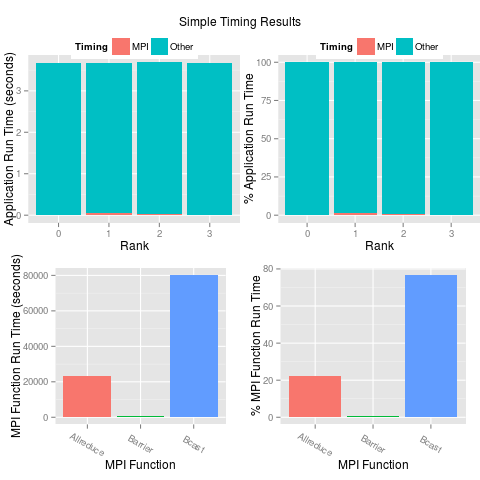
\includegraphics[scale=.39]{../common/pics/prof/timing.png}
\end{center}
  \end{block}
\end{frame}


\begin{frame}[fragile]
  \begin{block}{Generate plots}
  \begin{center}\vspace{-.6cm}
\begin{lstlisting}
plot(prof.data, plot.type="stats1")
\end{lstlisting}\vspace{-.2cm}
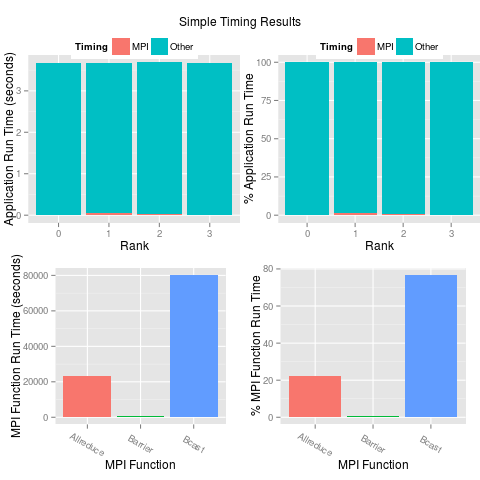
\includegraphics[scale=.39]{../common/pics/prof/timing.png}
\end{center}
  \end{block}
\end{frame}


\begin{frame}[fragile]
  \begin{block}{Generate plots}
  \begin{center}\vspace{-.6cm}
\begin{lstlisting}
plot(prof.data, plot.type="messages1")
\end{lstlisting}\vspace{-.2cm}
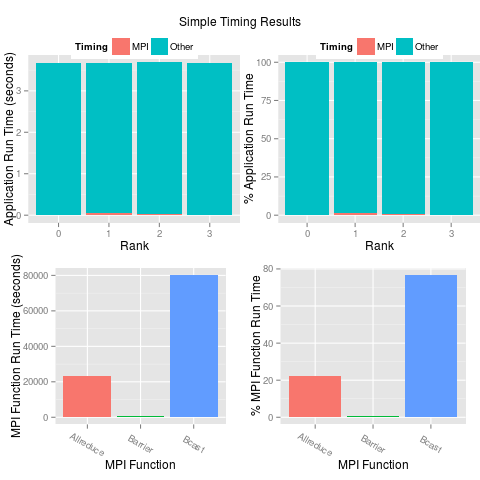
\includegraphics[scale=.39]{../common/pics/prof/timing.png}
\end{center}
  \end{block}
\end{frame}
